% NOTE: NO \documentclass, NO \begin{document}, NO \end{document} in this file!

\chapter{Biocrust-linked changes in soil aggregate stability along a climatic gradient in the Chilean Coastal Range}
\label{chap:manuscript1} % Label for potential cross-referencing (start page)

\section*{Abstract} % Use \section* for unnumbered sections if needed
Biological soil crusts (biocrusts) composed of cyanobacteria, bacteria, algae, fungi, lichens, and bryophytes stabilize the soil surface. This effect has mainly been studied in arid climates, where biocrusts constitute the main biological agent to stabilize and connect soil aggregates. Besides, biocrusts are an integral part of the soil surface under mediterranean and humid climate conditions, mainly covering open spaces in forests and on denudated lands. They often develop after vegetation disturbances, when their ability to compete with vascular plants increases, acting as pioneer communities and affecting the stability of soil aggregates. To better understand how biocrusts mediate changes in soil aggregate stability under different climate conditions, we analyzed soil aggregate samples collected under biocrust communities from four national parks in Chile along a large climatic gradient ranging from (north to south) arid (Pan de Azúcar), semi-arid (Santa Gracia), mediterranean (La Campana) to humid (Nahuelbuta). Biocrust communities showed a stabilizing effect on the soil aggregates in dry fractions for the three northern and the wet aggregates for the southernmost sites. Here, permanent vascular plants and higher contents of organic carbon and nitrogen in the soil control aggregate stability more than biocrusts, which are in intense competition with higher plant communities. Moreover, we found an increase in stability for aggregate size classes $<$\SI{2.0}{\milli\meter} and 9.5 – 30.0 mm. The geometric mean diameter of the soil aggregates showed a clear effect due to the climatic gradient, indicating that the aggregate stability presents a log-normal instead of a normal distribution, with a trend of low change between aggregate size fractions. Based on our results, we assume that biocrusts affect the soil structure in all climates. Their role in aggregate stability is masked under humid conditions by higher vegetation and organic matter contents in the topsoil.

\section{Introduction}
In recent years, biological soil crusts (biocrusts) have gained particular interest as stabilizers of soil aggregates. Such biocrusts are highly variable communities of microscopic (cyanobacteria, algae, fungi, and bacteria) and macroscopic (lichens, bryophytes) organisms found on the surface and in the upper centimeters of the soil (Gao et al., 2017). They stabilize the soil surface (Garcia-Pichel et al., 2016), especially in arid climates, where biocrusts are the main biological agents for consolidating and connecting soil aggregates (Belnap and Büdel, 2016). However, biocrusts are also present in more mesic regions (e.g., pine barrens, serpentine soils, temperate steppe) (Belnap et al., 2016), but due to their limited ability to compete for light, they are mainly relegated to open spaces or interspaces between vascular plants where sunlight reaches the soil surface (Malam Issa et al., 1999).

Because of their simple structure, biocrusts are present in a wide variety of climatic conditions. Biocrust organisms lack specialized desiccation control structures, such as stomata or impermeable cuticles, so their water content depends on the humidity in the surrounding environment (Thielen et al., 2021). However, low water demand, high drought tolerance (Chen et al., 2020), the ability to grow actively only when water is available, and to recover without physiological damage even after completely drying out for an extended period (Oliver et al., 2005) compensate the lack of dedicated structures. For this reason, biocrusts form an almost continuous layer in arid regions where water availability limits vascular plant cover (Colesie et al., 2014; Grote et al., 2010). By slightly increasing the water availability, areas covered by plants and biocrusts increase in self-organized patterns where both coexist. However, when water demand is no longer restrained, vascular plants have an advantage in using light due to their canopy development, which leads to a decline of biocrusts (Chen et al., 2018).

The cover and composition of biocrusts strongly depend on water availability (Bowker et al., 2016). Under dry conditions, with high potential evapotranspiration, biocrusts are dominated by cyanobacteria, bacteria, and micro-fungi, with few bryophytes or lichens present. However, the occurrence of lichens is not restricted to more humid locations, but lichens were also found in arid regions like Pan de Azucar in northern Chile (Jung et al., 2020b; Jung et al., 2020a). It implies that the external morphology of the biocrusts ranges from smooth to rugose (Chamizo et al., 2016). In terms of soil conditions, the water-holding capacity determines how much water can be stored in the soil. Typical sources of soil water are precipitation in general and, more specifically, at valley bottoms with close connection to the groundwater table, also groundwater. Further, available water for lichen growth can be provided by fog and dew (Jung et al., 2019). Pore space and pore size and following water-holding capacity of a soil largely depends on the parent material and its degree of weathering. Thus, soil formation indirectly controls the distribution and composition of biocrusts at ecoregional and local scales (Bowker et al., 2016). For instance, Steven et al. (2013) showed that the composition of biocrust communities differed at vertical scales of a few centimeters in soils with different parent material origins, while Bowker et al. (2016) concluded that heterogeneous distributions in parent materials result in abrupt transitions in biocrust distribution and cover.

Biocrusts can be understood as an organic-sedimentary system within the topsoil where the inorganic and the organic part play dynamic roles in determining the architecture, evolution, and properties of the system, including structure and aggregate stability. On a small spatial scale, biocrusts interact with the soil system in nitrogen and carbon cycling (Barger et al., 2016). Globally, Elbert et al. (2012) pointed out that cryptogamic covers take up 3.9 Pg C per year. The main processes of nitrogen enrichment are biological fixation and dust capture, while nitrogen losses typically appear via dissolution, volatilization, and erosional loss (Barger et al., 2016). Photosynthesis is the most crucial carbon fixation process (Elbert et al., 2012; Porada et al., 2014), and soil erosion and biological decomposition are the primary loss source of carbon and other nutrients (Li et al., 2008).

Biocrusts affect soil erosion by acting as a physical barrier that shields the soil from direct exposition to water and wind (Seitz et al., 2016), protecting it from the effect of raindrops and, thus, splash erosion (Seitz et al., 2017; Goebes et al., 2015) and modulating the abrasive effect of wind and surface runoff (Belnap and Büdel, 2016). At the same time, biocrusts control water flow across the landscape and through the soil matrix (Thielen et al., 2021; Eldridge et al., 2020). Eldridge et al. (2000) described a decrease in surface runoff and an increase in water infiltration in the presence of biocrusts under semi-arid conditions, related to a reduction in sediment discharge. The influence of biocrusts on the composition of the soil porosity is variable and depends on its stage of development and composition. In some cases, this structuration generates discontinuities that hinder the flow of water in the soil, while in others, it generates a decrease in the tortuosity that is reflected in rapid infiltration (Fischer et al., 2013). Water infiltration usually is inversely related to surface runoff (Lichner et al., 2012). The successional stage of biocrusts affects water repellency compared to bare soil (Drahorad et al., 2013). It has been observed that with the development of biocrusts, the water repellency increased, and the sorptivity and conductivity decreased (Fischer et al., 2012; Lichner et al., 2012). Therefore, biocrusts affect soil erosion and hydrology through a wide variety of processes (Belnap and Büdel, 2016).

In regards to the stability of the soil surface, biocrusts further have a binding effect on aggregates and can form coherent structures (Belnap and Büdel, 2016). Typically, the organic carbon in the form of exo-polysaccharides or structural filaments of the different organisms present within biocrust communities causes soil stabilization (Garcia-Pichel et al., 2016). Other structure-forming processes due to biocrusts, although to a lesser extent, are the compressive and drying action on the soil matrix and the pH-dependent dissolution of cementing salts (Bowker et al., 2016). The biocrusts-induced soil aggradation results in the formation of a defined layer, increasing the soil resistance and resilience to wind and water (Rosentreter et al., 2016).

Biocrusts stabilize individual aggregate units through different mechanisms depending on their species composition (Garcia-Pichel et al., 2016). For instance, bacteria, cyanobacteria, and also green-algae play a crucial role in forming and stabilizing aggregates by extracellular polymeric substances that glue soil particles together  (Six et al., 2004; Lewin, 1956). Vegetal debris serves as aggregation cores where the soil microorganisms use it as an energy source, but rapid decomposition is limited by the interaction with the inorganic matrix (Oades and Waters, 1991). On the other hand, fungi are important in forming soil aggregates due to their hyphal structure, which physically enmeshes microaggregates and soil particles (Totsche et al., 2018). In summary, soil aggregate stabilization processes are dynamic and occur at different temporal and spatial scales, where an aggregate of soil particles is built up of structural units of various sizes held together by various binding agents.

In this study, we investigate how and to what extent biocrusts under different climatic conditions stabilize the soil surface. Therefore, we compare the stability of macroaggregates and varying soil properties in topsoil with or without biocrust cover along a climatic gradient from arid to humid climate conditions along the Chilean Coastal Range. We test the following hypotheses:

\begin{enumerate}[label=(\roman*)] % Use lowercase Roman numerals in parentheses
    \item if biocrusts cover the soil surface, soil aggregates show higher stability because the biocrusts protect the soil surface physically, shelter soil organic matter within aggregates, modify the structure of microbial communities, and change water flow into the soil,

    \item if the climate is arid, the effect of biocrusts on the soil surface is most pronounced because other sources of organic matter are at minimum, and biocrusts represent the main soil cover, and

    \item if the humidity of the climate increases, the stabilizing effects of biocrust are reduced, although without disappearing entirely, because water availability increases and higher vegetation hinder the growth of biocrusts.
\end{enumerate}

\section{Materials and methods}
\subsection{Study sites and experimental settings}

In order to assess the climatic effect on soil and its interactions with biocrusts, four study sites distributed between latitudes from \ang{26;06}S to \ang{37;48}S and over 1300 km were established in the Chilean Coastal Range: Pan de Azúcar National Park (PA), Santa Gracia Natural Reserve (SG), La Campana National Park (LC) and Nahuelbuta National Park (NA), corresponding to arid, semi-arid, mediterranean and humid climates, respectively (Bernhard et al., 2018).

The study sites are comparable in geology, geomorphology, land use, and glacial and volcanic influence (Bernhard et al., 2018). The parent material in all the study sites is granitoid, keeping this factor of soil formation nearly constant along the studied gradient (Oeser et al., 2018). The dominant topography is generally fluvial valleys, and the sites had no glacial influence during the last glaciation (Hulton et al., 2002). The sites are located within nature protection areas, with limited anthropogenic influence compared to the surrounding areas. Despite this, the occasional entry of cows to LC (Rundel and Weisser, 1975) and goats to SG (Armesto et al., 2007) has been reported. These conditions allow us to focus on the environmental effect on two other soil-forming factors, i.e., climate and vegetation.

The mean annual temperature (MAT) decreases from north to south (PA: 16.8 °C, SG: 13.7 °C, LC: 14.1 °C, NA: 6.6 °C). The mean annual precipitation (MAP) in the study sites increases from north to south (PA: 12 mm yr-1, SG: 66 mm yr-1, LC: 367 mm yr-1, NA: 1469 mm yr-1) with similar rainfalls distribution mostly concentrated in winter months (May to August) (Bernhard et al., 2018). The elevation of the sites increases from north to south (PA: 329 – 351 m a.s.l., SG: 642 – 720 m a.s.l., LC: 708 – 732 m a.s.l., NA: 1200 – 1270 m a.s.l.). Paleoclimate modeling studies (Mutz et al., 2018) indicate that these climate patterns have been persistent since the late Pliocene; thus, the study sites represent the long-term impact of climate on the soil (Ewing et al., 2006). Bernhard et al. (2018) classified soils in the study sites as Regosols in PA, Cambisols for SG and LC, and Umbrisols in NA. In general, pedogenic processes such as soil depth, clay contents, organic matter accumulation, porosity, and activity ratio are correlated with the humidity of the site.

For each of the 4 study sites, 5 plots of 1 x 1 m were established as replicates. Each plot was located in the top-slope position with south-facing exposition, considering the presence of site-typical biological soil crust communities, similar slope and aspect, lack of anthropogenic disturbance, and a maximum distance of 30 m between each plot. Each plot included patches with at least the size of the samples with 100\% biocrust cover (BSC+), and additionally, a nearby point without biocrust cover (BSC-) was defined as control.

\subsection{Biocrust sampling and classification}

Biocrust patches of approximately 100 cm2 were identified according to Lange and Belnap (2016) and collected in the field by carefully detaching the biocrust layer, removing the loose soil, and storing it in paper envelopes after air-drying for every research plot. Samolov et al. (2020) describes the a biocrusts dominance in PA with cover of up to 40\%. The other study sites are dominated by higher vegetation that limits the cover of biocrust up to 15\% in SG and 5\% in LC and NA. Sampled communities showed all typical biocrust classes from cyanobacteria, algae, fungi, lichens, liverworts, and mosses. The species composition further showed a graduating change from lichen-dominating biocrusts in the northernmost site to bryophyte-dominating biocrusts in the southernmost site. Biocrusts in NA were specifically found in zones of forest soil disturbance. Bryophytes were sampled with rhizoids down to 5 mm depth; all other species were down to 2 mm. Dominant macroscopic biocrust species were determined for each of the four sites to the genus level by morphological characteristics using a stereomicroscope (Leitz TS, Wetzlar, Germany), a transmitted-light microscope (Leitz Laborlux S, Wetzlar, Germany), and ultraviolet light. Species groups were separated into bryophytes (Lightowlers, 1985; He, 1998; Ochyra and Matteri, 2001; Cuvertino et al., 2012; Fariña and Ardiles, 2014) and lichens (Galloway and Quilhot, 2009) and assigned to the different regions (Table 1). Baumann et al. (2018), based on morphological identification of enrichment cultures, reported that the biocrusts of all studied areas were composed of 18 to 15 species of algae and cyanobacteria; where the richness of green algae increased, while the richness of cyanobacteria decreased with increasing humidity and decreasing mean annual temperature. While Samolov et al. (2020), based on morphological and molecular traits, reported 18 species in PA, 26 species in SG, 40 species in LC, and 27 species in NA. A more detailed survey and classification of individual species, including algae and cyanobacteria, will be sought for further studies.

\begin{figure}[H]
	\centering
	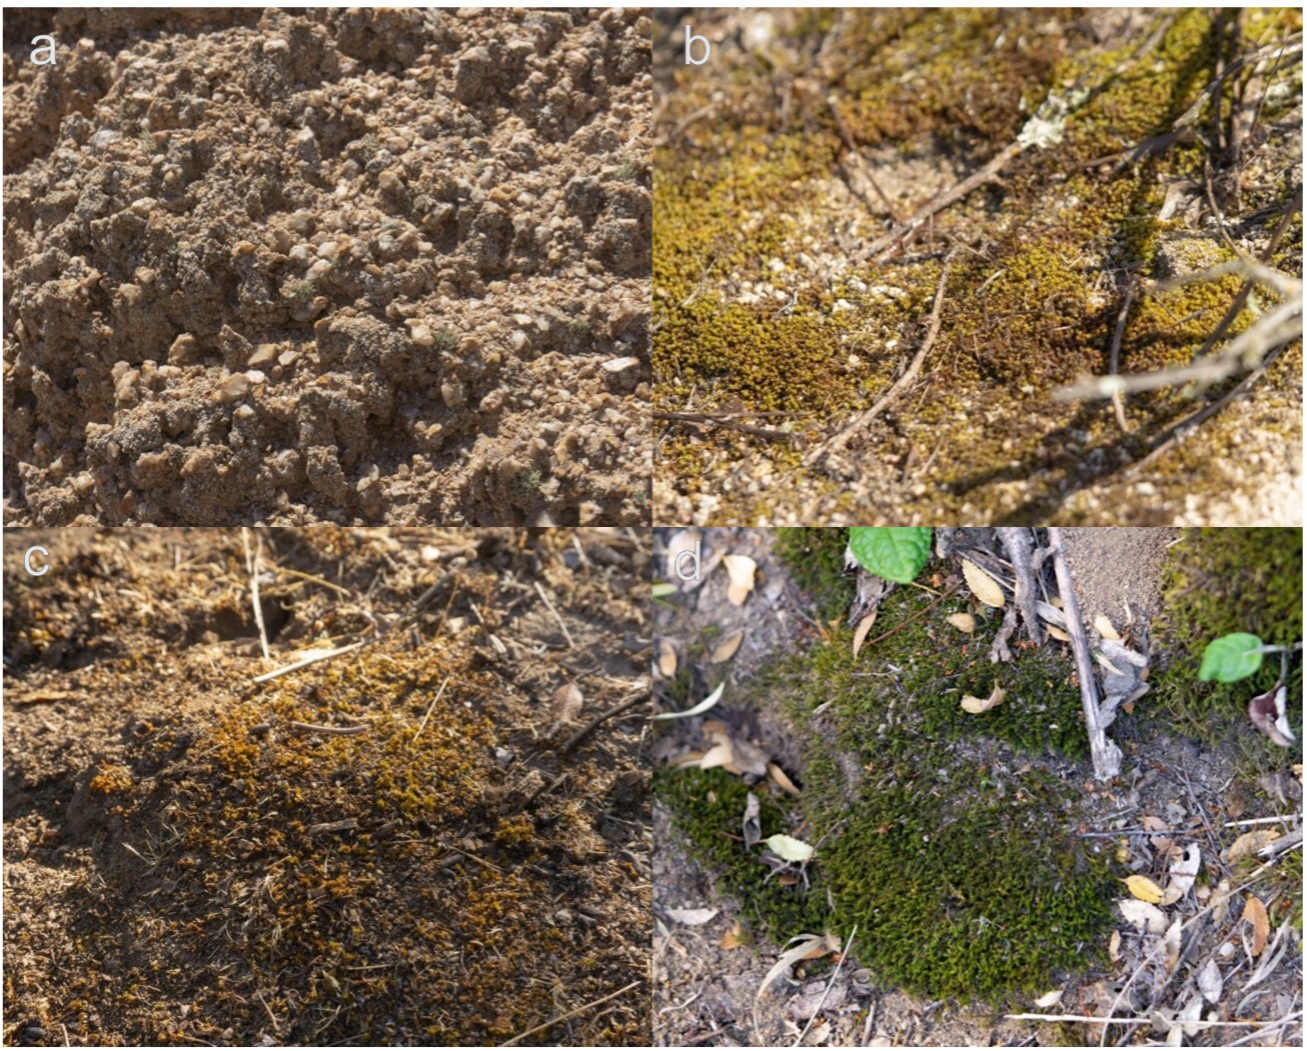
\includegraphics[width=1\textwidth]{img_hd/M1-Figure_1.png}
	\caption{Sampled biological soil crust for PA (a), SG (b), LC (c), and NA (d).}
	\label{fig:M1-F1-Sampled_biocrust}
\end{figure}

\FloatBarrier

\begin{table}[h!]
\centering
\caption{Taxonomical composition of mosses and lichens in the biological soil crust for the study sites along the climatic gradient.}
\resizebox{\textwidth}{!}{%
\begin{tabular}{lllc}
\hline
\textbf{Site / Division} & \textbf{Family} & \textbf{Genus} & \textbf{No. species} \\
\hline
\textbf{PdA} & & & \\
Lichens & Cladoniaceae & \textit{Cladonia} sp. & 2 \\
        & Verrucariaceae & \textit{Placidium} sp. & 2 \\
        & Lecanoraceae & \textit{Lecidella} sp. & 1 \\
        & Rhizocarpaceae & \textit{Rhizocarpon} sp. & 1 \\
\hline
\textbf{SG} & & & \\
Mosses & Pottiaceae & \textit{Syntrichia} sp. & 2 \\
       & Pottiaceae & \textit{Tortella} sp. & 2 \\
Unidentified lichens & & & 2 \\
\hline
\textbf{LC} & & & \\
Mosses & Bartramiaceae & \textit{Philonotis} sp. & 1 \\
       & Bryaceae & \textit{Bryum} sp. & 1 \\
       & Pottiaceae & \textit{Syntrichia} sp. & 2 \\
       & Pottiaceae & \textit{Tortella} sp. & 2 \\
Unidentified mosses and lichens & & & 2 + 1 \\
\hline
\textbf{NA} & & & \\
Mosses & Amblystegiaceae & \textit{Acrocladium} sp. & 1 \\
       & Amblystegiaceae & \textit{Amblystegium} sp. & 1 \\
       & Bartramiaceae & \textit{Bartramia} sp. & 1 \\
       & Bryaceae & \textit{Bryum} sp. & 1 \\
       & Dicranaceae & \textit{Campylopus} sp. & 2 \\
       & Pterigynandraceae & \textit{Myurella} sp. & 1 \\
Unidentified liverworts, lichens, fungi & & & 2 + 2 + 1 \\
\hline
\end{tabular}}
\label{tab:taxonomical_composition}
\end{table}

\FloatBarrier

\subsection{Soil sampling and analyses}

For soil characterization, bulk topsoil samples (0 – 5 cm) were taken with metal-core sample augers directly under biocrust patches and in comparative zones without biocrust cover and sieved to 2 mm after air drying. Bulk density (BD) and soil water content were determined gravimetrically. The particle size distribution was determined for seven fractions according to Köhn (1929), combining sieving of fractions >20 μm and pipetting of fractions <20 μm. Soil texture was interpreted according to the WRB soil classification system (Jahn et al., 2006). Soil pH was determined in water by a WTW pH 340 (WTW GmbH, Weilheim, Germany) using a Sentix 81 electrode, and electrical conductivity was measured with a conductivity meter (LE703, Mettler Toledo, USA). Total carbon (Ct) and nitrogen (Nt) of the bulk topsoil samples (0 – 5 cm) were analyzed using oxidative heat combustion at 1150 °C in a Vario EL III elemental analyzer (Elementar Analysensysteme GmbH, Hanau, Germany). Total organic carbon (TOC) was corrected by the carbonate content of samples with pH >6.7. The carbonate content was determined from the volumetric titration of the reaction with 10\% HCl using a calcimeter (Eijkelkamp, Giesbeek, Netherlands).

The physical stability of soil aggregates was measured to quantify the destructive effect of water and mechanical forces through two-stage sieving: dry and wet (Hartge and Horn, 2009). Water-stable aggregates were measured by sieving 200 g of undisturbed, air-dried soil samples, homogenized to 30.0 mm, through a stack of sieves of decreasing mesh size (19.0, 14.7, 9.8, 6.8, 4.8, 3.3, 2.0 mm, plus that collected the remainder below 2.0 mm) and then repeating the same process underwater (Six et al., 2000). Finally, coarse fragments (stones) were removed, and the values for each size were calculated relative to the weight of the initial sample. With this aggregate stability data, accumulated frequency curves were calculated, and a set of stability indexes were estimated: difference in mean weight diameter of the aggregates (ΔMWD) (Hartge and Horn, 2009; Van Bavel, 1950; Loaiza Puerta et al., 2018), difference in geometric mean diameter (ΔGMD) (Mazurak, 1950; Kemper and Rosenau, 1986), water stability aggregate ratio (WSAR) (Liu et al., 2014) and the proportion of soil macroaggregates of a diameter less than 2 mm (R<2 mm) (Liang et al., 2015) as described below. ΔMWD and ΔGMD indicate how much the average diameter of soil aggregates changes between dry and wet conditions. The main difference between ΔMWD and ΔGMD is that the first considers a linear behavior between the different aggregate size classes, while the ΔGMD considers a logarithmic fitting.

\subsubsection{Difference in mean weight diameter ($\Delta$MWD)}

    $$\Delta MWD = \frac{\sum_{i=1}^{n} X_i*W_i}{\sum_{i=1}^{n} W_i}$$
    where $W_i$ is the corrected mass proportion of stable aggregate fraction $i$ in the total 2–30 mm aggregate fractions, and $X_i$ is the mean diameter of stable aggregate fraction $i$. and $n$ is the number of particle fractions.

\subsubsection{Difference in geometric mean diameter ($\Delta$GMD)}
    $$\Delta GMD = exp \left[\frac{\sum_{i=1}^{n} X_i\lg W_i}{\sum_{i=1}^{n} W_i}\right]$$
    where $X_i$ is the sieve opening size (mm), $W_i$ is the proportion of the total sample mass occurring in the $i$-size fraction, and $n$ is the number of particle fractions.

\subsubsection{Water stability aggregate ratio (WSAR)}

    $$WSAR = \frac{WSA}{A}*100$$
    where $WSA$ is the >2 mm water-stable aggregate content, and  $A$ is the >2 mm dry aggregate content.

\subsubsection{Proportion of soil macroaggregate of a diameter less than 2 mm (R$_{<2mm}$)}
    $$R_{<2mm}=\frac{W_{r>2}}{W_T}*100 = \left(1-\frac{W_{r<2}}{W_T}\right)$$
    where $W_{r>2}$ is the weight of macroaggregates with a diameter less than 2 mm, $W_T$ is the total sample weight, $W_{r<2}$ is the weight of microaggregates with a diameter less than 2 mm.
    
\subsection{Statistical analyses}

The influence of the climatic gradient (study site) and biocrust presence on physicochemical soil parameters and aggregate stability in 40 plots (4 study sites, 2 biocrust treatments, 5 replicates) were assessed by factorial generalized linear models (GLM) because of the lack of normal distribution for most of the variables according to the Shapiro-Wilk test. The link functions used for each model were selected based on the lowest Akaike information criterion (AIC) selection and characteristics of the data (skewness, counts, continuous variables, proportions) between Gaussian, Gamma, inverse Gaussian, and Tweedie distributions. Differences in treatments were tested using Tukey post-hoc-test with $p <0.05$ as significance criteria. The analyses were conducted in R 4.2.0 (Team, 2018), and the GLM distributions were extended from the base R core with the Tweedie 2.3.3 package (Dunn, 2017). All visualizations were made with the package ggplot2 3.3.3 (Wickham, 2016)

\section{Results}
\subsection{Soil properties}

Soil pH was significantly affected by the climatic gradientError! Reference source not found.), with mean values of 7.7 in PA, 6.2 in SG, 5.9 in LC, and 4.4 in NA, with acidification levels of 6.2 in BSC- to 5.9 in BSC+. In terms of electrical conductivity (EC), a remarkably higher value of 2646.1 µS cm-1 in PA is outstanding in comparison with the low and homogeneous values of 109.3 µS cm-1 for SG, 153.8 µS cm-1 for LC, and 102.3 µS cm-1 for NA. EC did not differ for the biocrust treatment. Nevertheless, when looking at the site and biocrust in combination, the BSC+ results in a reduction of the EC in PA; meanwhile, in SG, LC, and NA there was no noticeable change. 

Bulk density (BD) showed a significant difference between the study sites, with higher values in the two dryer sites, with 1.5 g cm-3 in PA, and 1.6 g cm-3 in SG, and a decrease in the more humid sites, with 1.2 g cm-3 in LC and 0.6 g cm-3 in NA. Biocrust showed no changes for BD in SG and NA, but in PA BSC+ resulted in a reduction of the BD of 18.2%, while in LC BSC+ showed an increase in BD of 21.9% (Figure 2).

Total carbon (Ct) content was directly proportional to the humidity along the climatic gradient (Figure 2), with values of 1.1% in PA, 0.8% in SG, 5.0% in LC, and 12.5% in NA, but with a significant decrease when the BSC+ is present, from 5.6% to 4.2% in average. Soil inorganic carbon (SIC) was significantly higher in PA, with an average of 0.8% of the mass of the soil, while in SG, LC, and NA, it was not found. When looking at the SIC along the different sites and under biocrust in combination, the BSC+ results in a reduction of 70.1% in the SIC for PA, while in SG, LC and NA was no change. Soil organic carbon (SOC) showed a similar pattern as Ct, with a reduction in PA to 0.3% and the same 0.8% in SG, 5.0% in LC, and 12.5%. Total nitrogen (Nt) content was directly proportional to the humidity along the climatic gradient, with values of 0.04% for PA, 0.07% for SG, 0.28% for LC and 0.51% for NAError! Reference source not found.). BSC+ showed a reduction of 30.3% in LC and 22.3% in NA, while the Nt content remained stable in PA and SG under the influence of BSC. The relation between Ct and Nt, expressed as C/N, showed significantly different values of 33.9 in PA, 12.3 in SG, 16.7 in LC, and 24.5 in NA on average; and with a significant decrease from 27.0 in BSC- to 16.7 in BSC+ (Figure 2). It is important to note that although PA and NA present the highest values, the condition changes diametrically when observed together with the BSC+ treatment, with a large dispersion in PA and stable values in NA.

The distribution of the soil particle size classes did not show clear patterns along the climatic gradient, with PA deviating from it in all cases. Despite this, the observed values were significant, with clay values of 9.6% for PA, 7.3% in SG, 10.4% in LC, and 24.6% in NA, while when looking at the interaction between site and biocrust, there is an increase of 143.4% in clay content for the BSC+ condition, while for SG, LC and NA was no difference; silt with 28.9% in PA, 18.7% in SG, 20.0% in LC and 21.9% in NA; and sand with 61.5% in PA, 73.9% in SG, 69.6% in LC and 53.5% in NA. When biocrusts were present, a significant decrease from 13.6% to 12.6% in clays and an increase from 21.2% to 23.6% in silt was observed, with higher dispersion for the arid site (PA) (Figure 2Error! Reference source not found.).

\subsection{Soil aggregate stability}

Dry sieving showed a significant difference between study sites but not for the biocrust treatment (Figure 3). Dry aggregates in the 19.0 – 30.0 mm range showed significantly different values of 4.4% in PA, 1.2% in SG, 5.5% in LC, and 36.2% in NA. The fraction 9.5 – 19.0 mm revealed differences in the interaction between study sites and biocrusts, increasing the proportion of aggregates from 13.2% in PA to 19.3% SG and 29.3% in LC, not in NA with only 2.9% in the presence of biocrusts. The aggregates between 6.7 – 9.5 mm showed a significant decrease from 13.3% in PA, 5.2% in SG, 6.5% in LC, and 4.1% in NA. In interaction with biocrusts, it showed a significant increase in the proportion when it was present. The fraction from 4.7 – 6.7mm showed significantly different values of 13.6% in PA, 3.4 % in SG, 5.0% in LC, and 5.6% in NA, while the interaction with biocrusts showed a significant increase when is present (BSC+). Aggregates from 3.4 – 4.7 mm size showed significance among study sites, with 9.8% in PA, 3.6% in SG, 4.4% in LC, and 7.9% in NA. Aggregates between 2.0 – 3.4 mm showed a slightly similar amount of 9.9% in PA, 5.9% in LC, and 14.3% in NA, but with a minor proportion of 4.9% in LC, while when biocrust is present in LC, it showed a slight decrease. Finally, for the dry sieved aggregates under 2 mm, there was a significant reduction for the study sites, with values of 69.1% in SG and 47.3% in LC relative to 30.1% in PA, but not in NA with 28.9%; while the biocrust effect in interaction with the site is significant with 60.6% in SG and 40.8% in LC, indicating the same proportion of aggregates in this site for SG with 30.0% and NA with 39.8%.

In a second stage, aggregate stability under wet conditions was characterized, with a clear difference between sites, while biocrusts had a significant effect only on the aggregate size classes <2.0 mm and 9.5 – 30.0 mm (Figure 3). At the same time, the fraction 19.0 – 30.0 mm showed an increasing significant pattern in the amount of aggregates, with 2.8% in NA, 0.8% in SG, 8.9% in LC, and 29.9% in NA, while biocrusts significantly increased the proportion of aggregates by 35.6%, from 9.0% for BSC- to 12.2% for BSC+. For the fraction 9.5 – 19.0 mm, there were significant differences between the study sites, the biocrust effect, and its interactions, with an increase from 5.4% to 11.7% on average when biocrusts were present. The wet sieved aggregates in the range of 6.7 – 9.5 mm showed significant differences only between the study sites, with 10.6% in PA, 2.5% in SG, 4.2% in LC and 4.3% in NA. Wet aggregates in the range of 4.7 – 6.7 mm showed significant differences between the study sites with 10.6% in PA, 2.3% in SG, 3.7% in LC and 5.8 in NA. The fraction between 3.4 – 4.7 mm showed only significant differences between the study sites, with 6.9% in PA, 2.2% in SG, 3.0% in LC, and 6.1% in NA. Aggregates ranging from 2.0 – 3.4 mm showed differences between the study sites, with 5.8% in PA, 3.2% in SG, 4.2% in LC, and 6.8% in NA. The fractions under 2.0 mm were significantly different for the study sites, with 58.3% in PA, 79.6% in SG, 62.4% in LC, and 41.3% in NA; and for biocrusts from 63.9% for BSC+ treatment to 56.9% for BSC- treatment.

% Placeholder figure 3

When comparing the changes of the aggregate distributions between wet and dry conditions (Figure 4. Mean and standard deviation ), an irregular pattern was observed, with a general decrease in most of the analyzed fractions, except for an increase in the amount of aggregates of 19.0 mm for NA. This was even higher than for the BSC+ treatment. It is important to mention that NA also showed a slight increase in the proportion of 9.5 and 6.7 mm aggregates.

% Placeholder figure 4

Soil aggregate stability was evaluated through different indexes to integrate the different sizes and sieving conditions in a summary value. The difference in mean weight diameter of the aggregates (ΔMWD) showed no significance in any of the conditions (Figure 5). However, there was a significant difference in the difference of the geometric mean diameter of the aggregates (ΔGMD) for the study sites, with values of 1.86 mm for PA, 1.2 mm for SG, 1.4 mm for LC, in comparison with the more stable condition of 0.83 mm for NA. The water-stable aggregates ratio was significant for the study sites, showing differences between NA with 81.1% and the other study sites (57.7% PA, 66.2% SG, and 73.4% LC). The ratio of soil macroaggregates of a diameter less than 2.0 mm (R<2 mm) presents differences in the study sites and for biocrust treatments. SG showed a value of R<2 mm of 79.6% and NA of 41.9%, which was different from PA and LC, with 58.6% and 62.4%, respectively. For biocrust treatments, R<2 mm changed from 63.7% to 57.5% with biocrusts, indicating a biocrust-induced decrease in the proportion for this fraction. Finally, according to the analyzed indexes, NA showed the most stable conditions, and alternating PA and SG showed the most unstable conditions.

% Placeholder figure 5

As shown in Figure 2, the climatic gradient (site) had significant pH, electrical conductivity (EC), bulk density (BD), total carbon (Ct), soil organic carbon (SOC), soil inorganic carbon (SIC), total nitrogen (Nt), C/N, clay, silt, sand, dry and wet aggregates under 30 mm, ΔGMD, WSAR, R<2 mm. Biocrust treatments were significant for clay, silt, pH, EC, Ct, SOC, SIC, Nt, C/N, and wet aggregates from 9.5 to 30.0 mm and >2 mm, and R<2 mm. Finally, the interaction of the site and biocrusts was significant for clay, bulk density (BD), total nitrogen (Nt), dry aggregates from 4.7 to 19.0 mm and 0 to 3.4 mm, wet aggregates from 9.5 to 30.0 mm, and ΔMWD.

\section{Discussion}

\subsection{Aggregate stability and soil properties along the climatic gradient}

The climatic gradient has a significant effect on the stability of soil aggregates. Using the geometric mean diameter (ΔGMD), an index that replaces the linear fitting of ΔMWD with a logarithmic one, significant differences for the study sites along the climatic gradient can be observed (p-value: <0.001). When soil aggregate stability was evaluated with the difference in mean weight diameter (ΔMWD), it did not show significant changes along the climatic gradient. WSAR, an index that shows the ratio of aggregates that persist stably after disruption by water, showed a similar behavior as ΔMWD. The main difference between ΔMWD and ΔGMD is that ΔGMD performs better in non-uniform particulate substances (Hatch and Choate, 1929; Gardner, 1956), which corresponds to soils equilibrated in the content of sand, silt, and clay (Mazurak, 1950) and pointing soil texture indirectly as a critical factor in aggregate stability along the climatic gradient. Further, considering the ΔGMD data, an increase in stability was observed as moving along the climatic gradient to higher water availability conditions except for SG. The lower value of ΔGMD for SG indicates comparably higher aggregate stability as it would be expected when we assume a steady trend from arid to humid climate. In PA, in the drier north, the condition proved to be less stable than NA, despite the high content of inorganic carbon. SG presented the highest ratio of unstable aggregates under the studied range of sizes (highest R<2mm) and NA the lowest, with close to half of it, indicating augmented aggregate stability in the complementary range of sizes.

The effect of the climatic gradient is not only expressed in the stability of soil aggregates, but it is also present with different intensities in a variety of soil properties. The pH decreases continuously from the northern arid to the southern humid study site in accordance with Bernhard et al. (2018). The high pH in PA can be attributed to the constant input of atmospheric aerosols, e.g., salts, gypsum, and calcium carbonates (Ewing et al., 2006) in combination with the arid climate that allows salts to accumulate in the topsoil (Slessarev et al., 2016). Whereas in the southern sites, the forwarding increase of precipitations results in a reduction in the pH due to leaching of soluble salts (Slessarev et al., 2016) and an increase in soil respiration (Orchard and Cook, 1983). The accumulation of soluble salts is well established for the arid site PA, as saline conditions (Allison and Richards, 1954) are indicated by the high electrical conductivity value. These higher amounts of salts have a strong effect in structure degradation dynamics, linked to the destabilizing effect of sodium and stabilizing of carbonates (Corwin, 2021). Although Ct and Nt follow the climatic gradient, when comparing the C/N, PA and NA have higher values. High values of the C/N indicate a nitrogen limitation of plants and other organisms (Brust, 2019), pointing out that this occurs at the two opposite sites along the climatic gradient. This could be explained by the biological activity (Zhang et al., 2013), which may be close to a physiological limitation in the case of NA, while for PA, it may indeed be due to low nitrogen availability (Hooper and Johnson, 1999). However, there was also a high amount of carbonates in PA, which makes PA hardly comparable in terms of Ct. Despite the properties following the climatic gradient, SG deviates from the other sites in terms of higher bulk density (BD), lower clay, and higher sand content. This can indicate a degraded condition for the semi-arid site caused by the current land use, including grazing (Armesto et al., 2007), compacting the surface and thus activating erosive processes (Scholten and Seitz, 2019), in favor of the accumulation of sand particles (Govers, 1985). The aggregate distribution stresses this finding, where SG has a lower proportion of water-stable aggregates >2 mm and a higher water-destabilization of aggregates between 9.5 to 4.7 mm, indicating that the nature of the structuring agent in that zone is water-soluble.


\subsection{Biocrusts altering soil properties along the climatic gradientt}

Despite these factors beyond the climatic gradient, biocrusts showed effects on clay, silt, pH, Ct, Nt, C/N, and wet aggregates from 9.5 to 30.0 mm and >2 mm. However, as this was an observational study, it only allows establishing associations between factors and not cause-effect relationships (Cox, 1992; Rosenbaum, 2005). It is thus possible that changes in soil characteristics promote the biocrust establishment, as well as that biocrust establishment triggers changes in these properties (Belnap and Lange, 2003).

The biocrust treatments showed a significant decrease in pH (p-value: 0.002404), reflecting the biological activity of its constituent organisms, which acidifies the soil due to the carbon dioxide released by cellular respiration (Bachar et al., 2010). The pH values reported by Bernhard et al. (2018) are in the same range as ours but without differentiating between BSC+ and BSC-, as this factor was not part of their study. The content of Ct and Nt were significantly different when biocrusts were present, but it did not affect any aggregate sizes or stability indexes. In this sense, biocrusts play a role in the carbon and nitrogen cycles (Chen et al., 2000), as they are formed mainly by photosynthetic and nitrogen-fixing organisms (Maestre et al., 2013), but it has not had an immediate impact on the soil aggregate stability and points out that the primary stabilizing agent is of organic origin (Wagner et al., 2007; Six et al., 2004).

Considering the stabilizing effect of biocrusts on wet sieved aggregates between 9.5 and 30.0 mm, we could show that it occurs prominently at the three northern sites, whereas in NA there was no difference with and without biocrusts. This points to a threshold in the biocrust-induced stabilization of the soil aggregates between LC and NA and partially confirms our initial assumption that biocrusts have the greatest effect in arid conditions. However, the effect on aggregate stability for the wet condition varies according to the variable used, being specific for limited aggregate sizes in terms of mechanical disturbances (dry sieving) but without a substantial improvement concerning water stability (wet sieving). This lack of difference in wet sieved aggregate point to a non-soluble nature of the stabilizing agents, which can be attributed to stabilization due to organic structures and exudates (Rillig, 2004), and stress the idea that NA differs to the other sites in the mechanisms of aggregate stabilization as a local adaptation, where due to the higher proportion of precipitation, is conducted by water stable mechanisms.

Soil aggregate stability showed clear differences along the climatic gradient. However, when considering the effect of biocrusts, differences were limited to the smallest aggregate size class (R<2mm) referring to changes in microaggregates size distribution as described by Totsche et al. (2018). Further, a difference for wet sieved aggregates with and without biocrusts between 9.5 and 30.0 mm point to biocrust-induced stabilization of soil aggregates.

The results indicate that soil aggregate stabilization mechanisms are different in PA than at the other sites. With that in mind, it was found that in PA, biocrusts grow in areas with a lower content of clay and higher content of silt, which implies increased nutrient availability and water-holding capacity (Chen et al., 2000), while the sand fraction was not related. However, the method used can amplify that difference since the determination of particle size distribution does not consider coarse fragments (Köhn, 1929), which were abundant at PA. In addition, the soil covered with biocrusts showed a lower value for bulk density (BD) only for PA, while in the other sites, this property was not affected. This can be interpreted as a biocrust-induced decrease in soil density due to increased intra- and extra-aggregate porosity and organic matter (Whitney et al., 2017) or that biocrusts grow under the least limiting condition (Bowker et al., 2014). Soils with biocrust cover showed a trend of lower electrical conductivity, which can be explained by the inhibition of biocrusts by toxicity due to the accumulation of salts in the soil, or to the consumption of salts as a source of nutrients by the organisms in the biocrusts (Abed et al., 2019).

Biocrust plays a role along the climatic gradient affecting different properties, i.e., clay, silt, pH, Ct, Nt, C/N, and wet aggregates from 9.5 to 30.0 mm and >2 mm. Nevertheless, the way that each property change responds to local conditions: In the arid northernmost site, there is a strong influence of the salts in terms of stabilization and establishment of biocrusts, while at the southernmost site, there is no stabilization of the aggregates, but a contribution to the carbon and nitrogen contents. The most consistent property along the climatic gradient was pH, an indicator of biological activity. However, at the scale of the climatic gradient it is not possible to distinguish the origin of biological activity between plants, microorganisms, fungi, bacteria, etc. Finally, considering the largest size of the persistent wet aggregates match the characteristics attributed to fungi and bryophytes, capable of retaining micro-aggregates and soil particles between their hyphae and rhizoids, respectively (Kleber et al., 2007; Six et al., 2004; Totsche et al., 2018) and points to this as the most significant mechanism of soil aggregate stabilization of biocrusts.

\section{Conclusions}

This study aimed to investigate how and to what extent biocrusts stabilize soil aggregates along an arid to humid climatic gradient in Chile. We show that biocrusts play a role in soil aggregate stability along the climatic gradient by increasing the stability for wet aggregates from 9.5 to 30.0 mm and >2 mm. Bicorusts also modify other soil properties such as Ct, Nt, C/N, clay, and sand, indicating an initial accumulation of organic matter that then give place to aggregation processes. The biocrusts effect on aggregates stability was lower under humid climate conditions, which indicates a transition in the main biotic agents driving the aggregation of the soil surface, moving from biocrust communities in arid regions to vascular plants in humid conditions.
Finally, we conclude that the biocrusts in our study area showed to be a valuable agent in stabilizing the upper topsoil layer, but for a narrow spectrum of conditions and mostly under arid conditions. Therefore, the effect could be considered a transition in ecological succession toward a stable ecosystem. In this process, biocrusts improve conditions for other more demanding species, such as vascular plants, initially improving the availability of carbon and nitrogen in the soil.

\section*{Appendices}

\begin{table}[htbp] % [htbp] placement specifier (Here, Top, Bottom, Page)
\centering % Center the table on the page
\caption{Appendix A. Significant factors for response variables based on generalized linear models. Models with significant interaction also include the predictors as simple parameters based on marginality principle. \\ % Line break in caption
\textit{(p-value $\le$ 0: "***"; p-value $\le$ 0.001: "**"; p-value $\le$ 0.01: "*")}} % Significance key (using <= for clarity)
\label{tab:appendix_a} % Label for cross-referencing
\begin{tabular}{@{}lllll@{}} % Left-aligned columns, @{} removes extra space at edges
\toprule
Dependent variable & Distribution & \multicolumn{3}{c}{Significance for independent variable} \\
\cmidrule(lr){3-5} % Rule under the multicolumn header only (trimmed left and right)
 & (link-function for GLM) & Site & Biocrust & Site $\times$ Biocrust \\ % Use $\times$ for multiplication
\midrule
Clay	& Gaussian	& ***	& *	& \\
Silt	& Inverse Gaussian	& ***	& *	& \\
Sand	& Gaussian	& ***	& 	& \\
Fine Silt	& Tweedie	& ***	& 	& * \\
Medium silt	& Tweedie	& ***	& ***	& * \\
Coarse silt	& Tweedie	& ***	& 	&  \\
Very fine sand	& Gaussian	& ***	& 	&  \\
Fine sand	& Tweedie	& ***	& 	&  \\
Medium sand	& Gaussian	& ***	& 	&  \\
Coarse sand	& Tweedie	& ***	& 	&  \\
pH	& Gaussian	& ***	& **	&  \\
EC	& Tweedie	& ***	& 	&  \\
BD	& Gaussian	& ***	& 	& ** \\
N\textsubscript{t}	& Gamma	& ***	& 	& ** \\ % For Nt subscript
C\textsubscript{t}	& Tweedie	& ***	& **	&  \\ % For Ct subscript
C/N	& Tweedie	& ***	& **	&  \\
19.0-30.0 mm Dry	& Tweedie	& ***	& 	&  \\
9.5-19.0 mm Dry	& Tweedie	& ***	& 	& ** \\
6.7-9.5 mm Dry	& Tweedie	& ***	& 	& ** \\
4.7-6.7 mm Dry	& Tweedie	& ***	& 	& * \\
3.4-4.7 mm Dry	& Tweedie	& ***	& 	&  \\
2.0-3.4 mm Dry	& Tweedie	& ***	& 	& * \\
\textless2.0 mm Dry	& Tweedie	& ***	& 	& *** \\ % Use \textless for less than symbol
19.0-30.0 mm Wet	& Tweedie	& ***	& *	& ** \\
9.5-19.0 mm Wet	& Tweedie	& *	& **	& * \\
6.7-9.5 mm Wet	& Tweedie	& ***	& 	&  \\
4.7-6.7 mm Wet	& Tweedie	& ***	& 	&  \\
3.4-4.7 mm Wet	& Tweedie	& ***	& 	&  \\
2.0-3.4 mm Wet	& Tweedie	& ***	& 	&  \\
\textless2.0 mm Wet	& Tweedie	& ***	& *	&  \\ % Use \textless for less than symbol
$\Delta$MWD	& Gaussian	& 	& 	&  \\ % Use \Delta for Greek Delta
$\Delta$GMD	& Tweedie	& ***	& 	&  \\ % Use \Delta for Greek Delta
WSAR	& Gaussian	& 	& 	&  \\
R\textless2 mm	& Gaussian	& ***	& *	&  \\ % Use \textless for less than symbol
\bottomrule
\end{tabular}
\end{table}

\FloatBarrier

\section*{Data availability}

The data that support the findings of this study are available from the corresponding author upon request.

\section*{Code availability}

The code that supports the findings of this study are available from the corresponding author upon request.

\section*{Author contribution}

TS, DW, CWM, OS, and StS conceptualized the study. OS, KW, and NRM collected the soil samples. StS collected and analyzed the biocrust samples, and NRM analyzed the soil samples. NRM performed the analyses and prepared the manuscript.

\section*{Competing interests}


The authors declare that they have no conflict of interest.

\section*{Acknowledgments}

We are deeply grateful to the students, technical assistants, and colleagues who helped in the field and laboratory phases. A special thanks to Martin Nebel and Sonja Thielen for their help in classifying bryophytes and lichens. Oliver Burkhardt (GFZ German Research Centre for Geosciences) and Franziska Steiner (Technical University of Munich) for their support in the field. Hugo Pérez for his help and experience in the soil physics laboratory of the Universidad de Chile. We are grateful to the Chilean National Forest Corporation (CONAF) and Sucesión Gálvez Muñoz, who provided access to the study sites. The study was funded by the German Science Foundation DFGSPP 1803 (EarthShape; www.earthshape.net). We acknowledge support by Open Access Publishing Fund of University of Tübingen. 
